\chapter{Основы шифрования. Симметричные шифры} \label{chapt1}%
\textbf{Мета роботи:~}%
Изучить основные типы шифров. Исследование симметричных методов шифрование.
Получение практических навыков изученных методов шифровки сообщений.

\section{Теоретические ведомости} \label{sect1_a}
%
Криптография представляет собой совокупность методов преобразования данных,
направленных на то, чтобы сделать эти данные бесполезными для злоумышленника.
Такие преобразования позволяют решить два главных вопроса, касающихся
безопасности информации:
\begin{itemize}
  \item защиту конфиденциальности;
  \item защиту целостности.
\end{itemize}

Проблемы защиты конфиденциальности и целостности информации тесно связаны
между собой, поэтому методы решения одной из них часто применимы для решения
другой. %
%%%   https://www.rutvet.ru/in-metody-i-vidy-kriptografii-i-shifrovaniya-dlya-nachinayushchih-8728.html
%\paragraph{Современная криптография}%

\paragraph{Виды криптосистем}%
Для многих обывателей термин «криптография» означает что-то загадочное и
таинственное. Однако в настоящее время различные виды шифрования можно
встретить буквально везде — это и простые кодовые замки на дипломатах, и
многоуровневые системы защиты секретных файлов. Люди сталкиваются с ней,
когда вставляют в банкомат карточку, совершают денежные переводы, покупают
через интернет товары, общаются по Skype, отправляют письма на электронную
почту. Любые дела, связанные с информацией, так или иначе имеют отношение к
криптографии. Но, несмотря на всё многообразие сфер применения, в настоящее
время существует всего несколько способов шифрования. Все эти методы
криптографии относятся к двум видам криптографических систем: симметричным (с
секретным ключом) и ассиметричным (с открытым ключом).
\subparagraph{Симметричный метод} %
Симметричные системы позволяют шифровать и расшифровывать информацию с
помощью одного и того же ключа. Расшифровать криптографическую систему
секретного ключа невозможно, если дешифровщик не обладает секретным ключом.

\subparagraph{Асимметричный метод}%
В криптографических системах с открытым ключом пользователи обладают
собственным открытым и частным закрытым ключами. К открытому ключу имеют
доступ все пользователи, и информация шифруется именно с его помощью. А вот
для расшифровки необходим частный ключ, находящийся у конечного пользователя.
В отличие от криптограмм с секретным ключом в такой системе участниками
являются не две, а три стороны. Третья может представлять собой сотового
провайдера или, например, банк. Однако эта сторона не заинтересована в
хищении информации, поскольку она заинтересована в правильном
функционировании системы и получении положительных результатов.

\subparagraph{Блочные шифры}%
%%http://bit.nmu.org.ua/ua/student/metod/cryptology/%D0%BB%D0%B5%D0%BA%D1%86%D0%B8%D1%8F%205.pdf
%
%
%%% https://studfiles.net/preview/1503566/
Это функция шифрования, которая применяется к блокам текста фиксированной
длины. Текущее поколение блочных шифров работает с блоками текста длиной 256
бит (32 байт). Такой шифр принимает на вход 256-битовый открытый текст и
выдаёт 256-битовый шифрованный текст.

Блочный шифр является обратимым: существует функция дешифрования, которая
принимает на вход 256-битовый шифрованный текст и выдаёт исходный 256-битовый
открытый текст. Открытый и шифрованный текст всегда имеет один и тот же
размер, который называется размером блока \emph{(block size)}.

%%% ANALYSIS OF THE DVB COMMON SCRAMBLING ALGORITHM, 2004
%% https://eprint.iacr.org/eprint-bin/cite.pl?entry=2004/289
\begin{figure}[!ht]
  \centering
  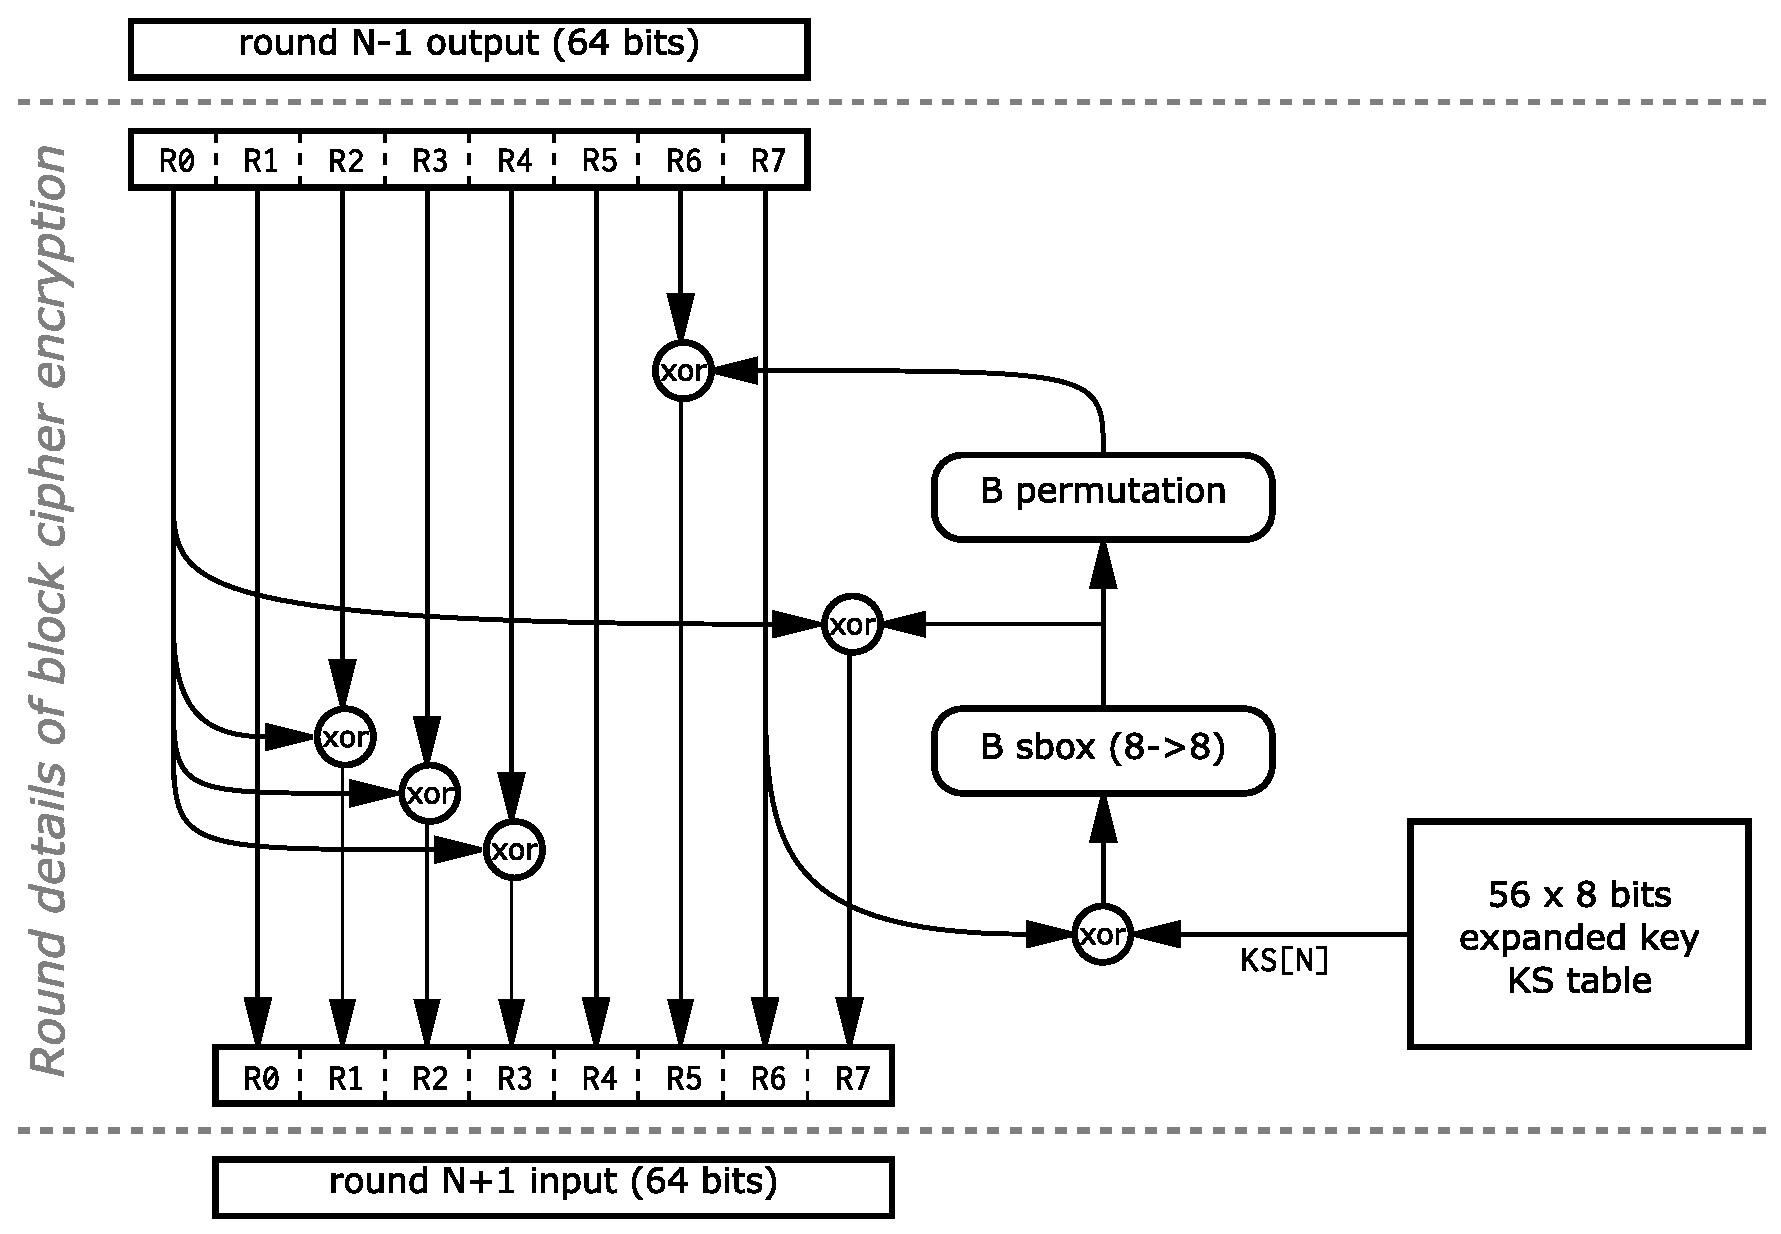
\includegraphics[width=\columnwidth/10*7]{Dvbcsa_block_encrypt}
  \caption{Подробный разбор алгоритма блочного скремблирования DVB }\label{Dvbcsa_block}
\end{figure}

\subparagraph{Потоковые шифры}%
Потоковые шифры представляют собой разновидность гаммирования и преобразуют
открытый текст в шифрованный последовательно по 1 биту. Генератор ключевой
последовательности выдаёт последовательность бит $k_1,k_2, \ldots,k_i, \ldots
$ Эта ключевая последовательность складывается по модулю 2 с
последовательностью бит исходного текста $p_1,p_2, \ldots,p_i, \ldots $ для
получения шифрованного текста:

\begin{equation}\label{potocShifr}
c_i=p_i \oplus k_i;
\end{equation}
На приемной стороне шифрованный текст складывается по мо­дулю 2 с идентичной
ключевой последовательностью для получения исходного текста:

\begin{equation}\label{potocShifr}
c_i \oplus k_i =p_i \oplus k_i \oplus k_i=p_i;
\end{equation}

%%% ANALYSIS OF THE DVB COMMON SCRAMBLING ALGORITHM, 2004
\begin{figure}[!ht]
  \centering
  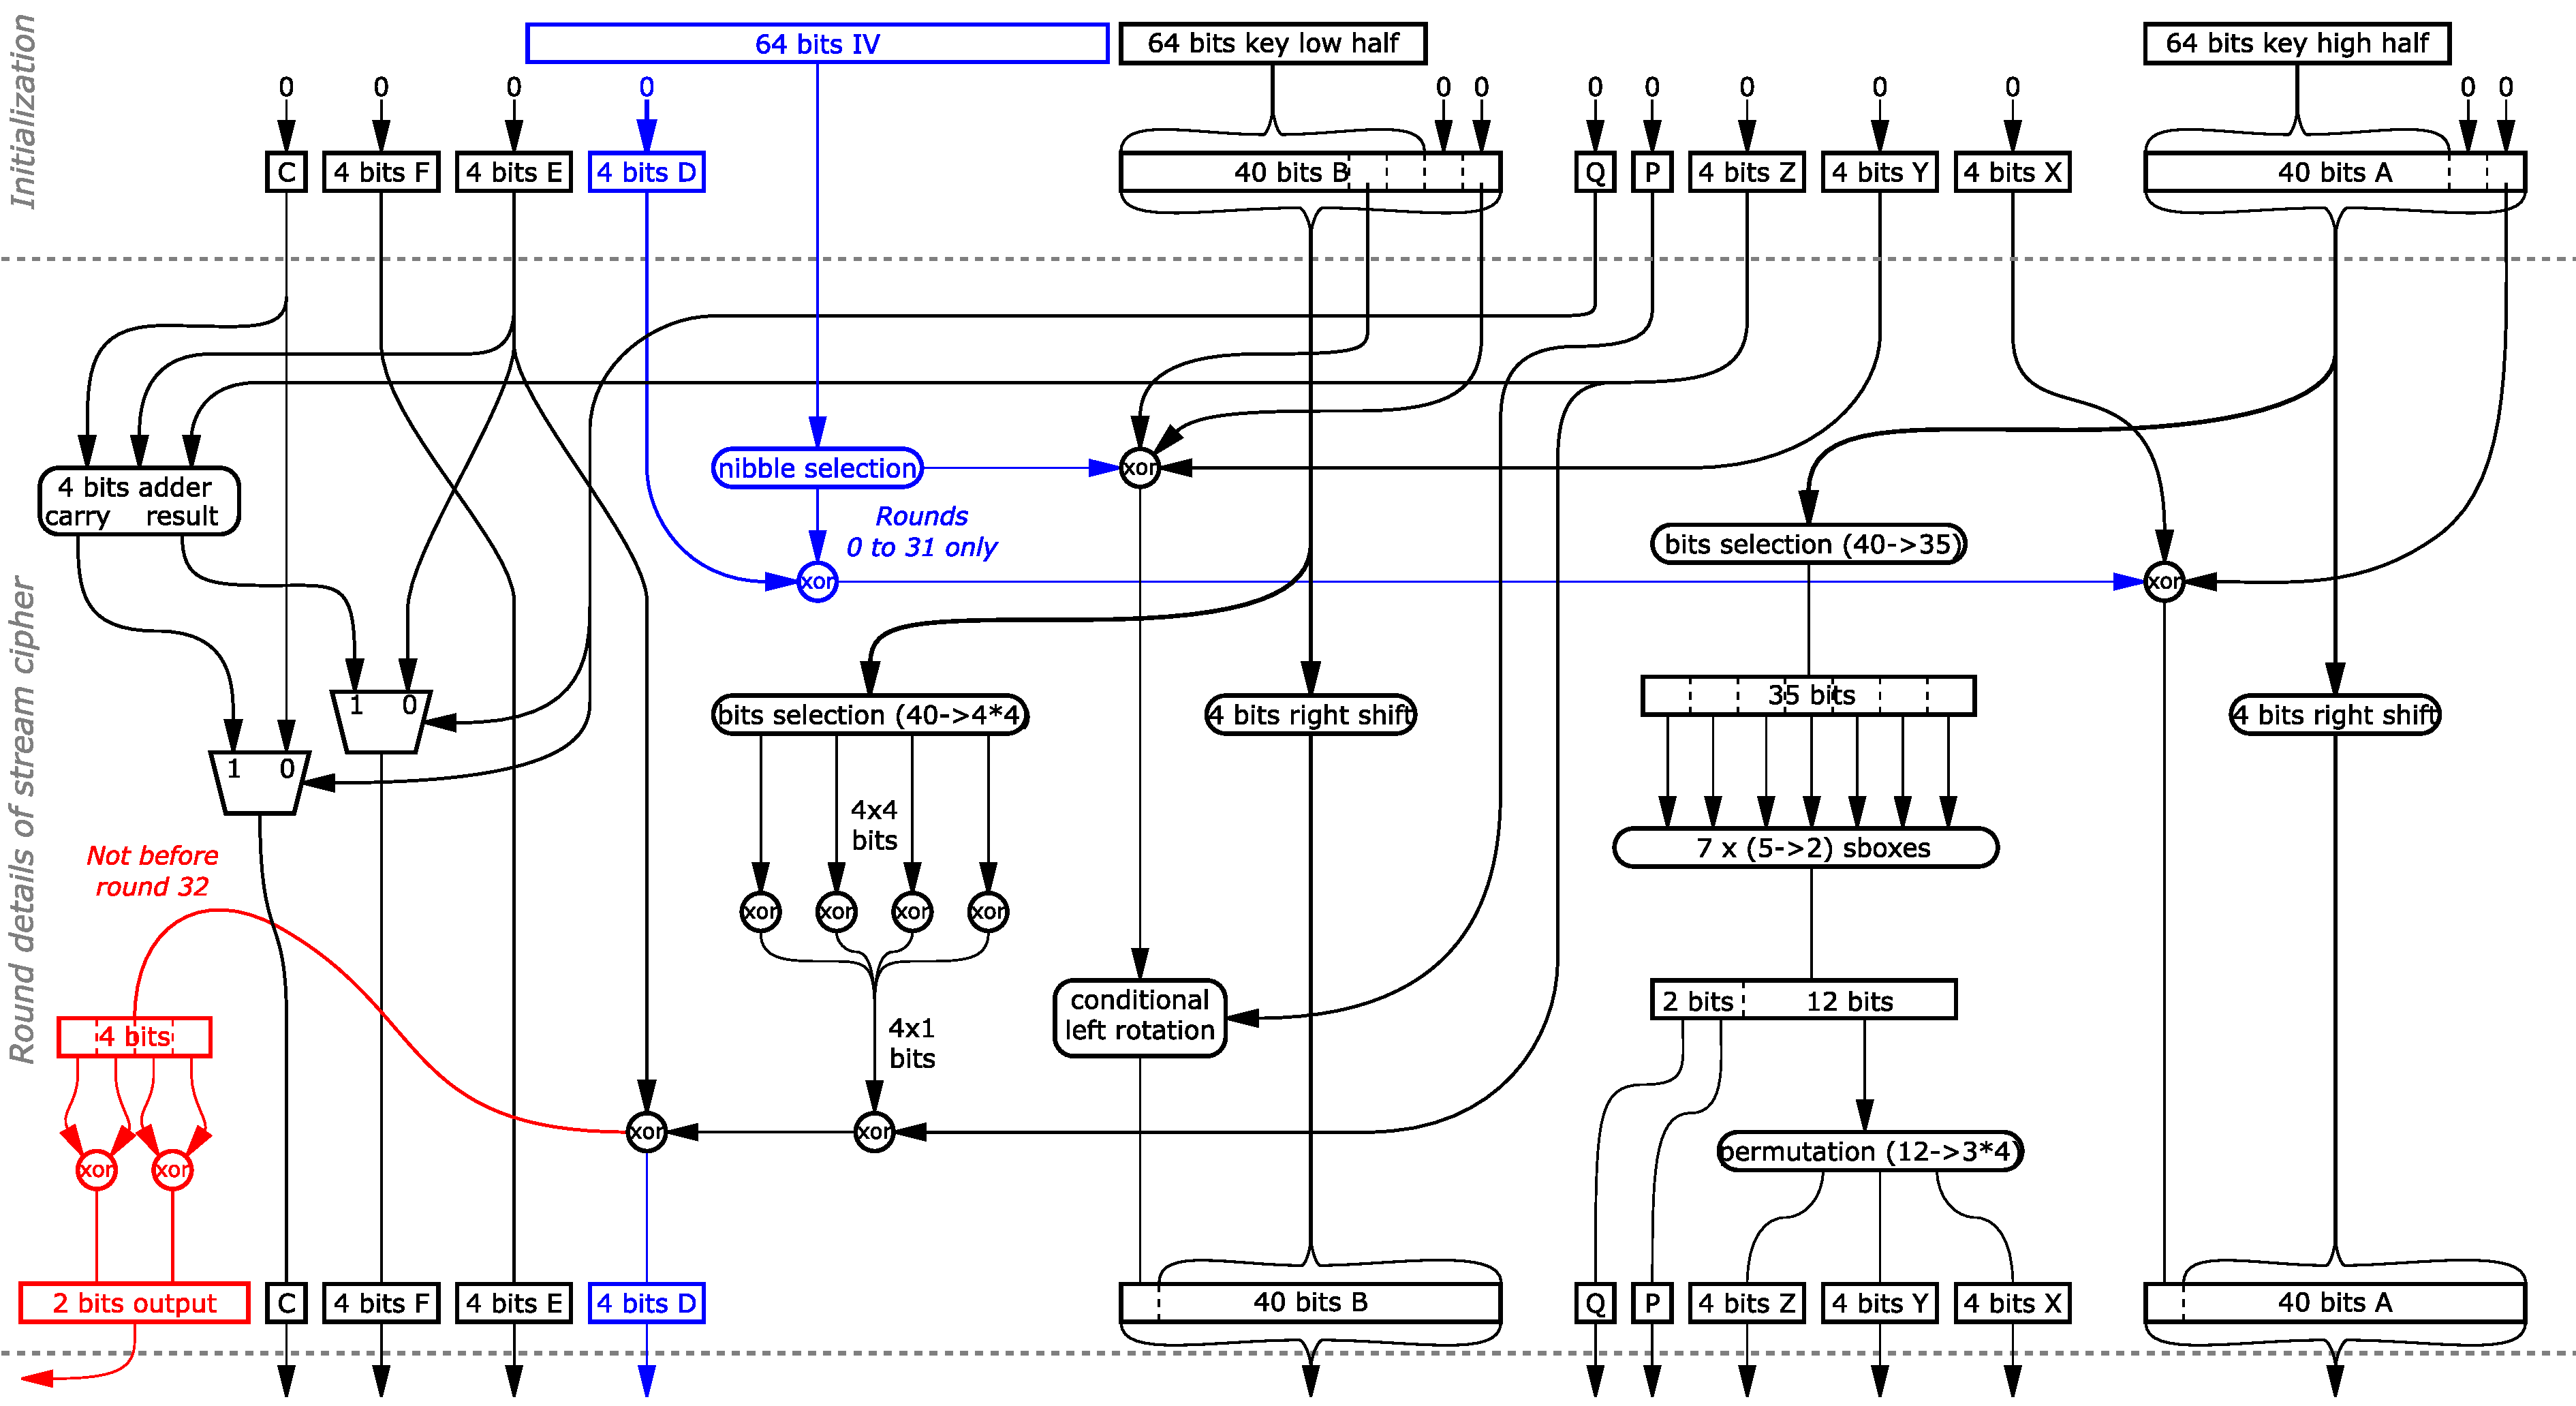
\includegraphics[width=\columnwidth]{Dvbcsa-stream}
  \caption{Подробный разбор алгоритма потокового скремблирования DVB }\label{Dvbcsa_stream}
\end{figure}
%%% https://studfiles.net/preview/1464213/
Стойкость системы целиком зависит от внутренней структуры генератора ключевой
последовательности. Если генератор выдаёт последовательность с небольшим
периодом, то стойкость системы будет невелика. Напротив, если генератор будет
выдавать бесконечную последовательность истинно случайных бит, то мы получим
«ленту однократного использования» с идеальной стойкостью.

Реальная стойкость потоковых шифров лежит где-то посредине между стойкостью
простой моноалфавитной подстановки и «ленты однократного использования».
Генератор ключевой последовательности выдаёт поток битов, который выглядит
случайным, но в действительности является детерминированным и может быть в
точности воспроизведен на приемной стороне. Чем больше генерируемый поток
похож на случайный, тем больше усилий потребуется от криптоаналитика для
взлома шифра.

\subparagraph{Криптографические протоколы} %
В современной криптографии большое внимание уделяется не только созданию и
исследованию шифров, но и разработке криптографических протоколов.

\textbf{Протокол} --- это последовательность шагов, которые предпринимают две
или большее количество сторон для совместного решения задачи. Все шаги
следуют в порядке строгой очередности, и ни один из них не может быть сделан
прежде, чем закончится предыдущий. Кроме того, любой протокол подразумевает
участие, по крайней мере, двух сторон.

%https://www.intuit.ru/studies/courses/691/547/lecture/12371?page=4
\textbf{Криптографический протокол} --- это такая процедура взаимодействия
двух или более абонентов с использованием криптографических средств, в
результате которой \emph{абоненты} достигают своей цели, а их
\emph{противники} -- не достигают. В основе протокола лежит набор правил,
регламентирующих использование криптографических преобразований и алгоритмов
в информационных процессах. Каждый криптографический протокол предназначен
для решения определённой задачи.

Рассмотрим простейший протокол для обмена конфиденциальными сообщениями между
двумя сторонами, которые будем называть \texttt{абонент №1} и \texttt{абонент
№2}. Пусть \texttt{абонент №1} желает передать зашифрованное сообщение
\texttt{абоненту №2}. В этом случае их последовательность действий должна
быть следующей.
\begin{enumerate}
  \item Абоненты выбирают систему шифрования \emph{(например, шифр
      Цезаря)}.
  \item Абоненты договариваются о ключе шифрования.
  \item \texttt{Абонент №1} шифрует исходное сообщение с помощью ключа
      выбранным
      методом
      и получает зашифрованное сообщение.
  \item Зашифрованное сообщение пересылается \texttt{абоненту №2}.
  \item \texttt{Абонент №2} расшифровывает зашифрованное сообщение с помощью
      ключа и
      получает открытое сообщение.
\end{enumerate}
Этот протокол достаточно прост, однако он может действительно использоваться
на практике. Криптографические протоколы могут быть простыми и сложными в
зависимости от назначения.

\paragraph{Сферы применения криптографии.}%
В настоящее время криптография прочно вошла в нашу жизнь. Перечислим лишь
некоторые сферы применения криптографии в современном информатизированном
обществе:
\begin{itemize}
  \item шифрование данных при передаче по открытым каналам связи (например,
      при совершении покупки в Интернете сведения о сделке);
  \item обслуживание банковских пластиковых карт;
  \item хранение и обработка паролей пользователей в сети;
  \item сдача бухгалтерских и иных отчётов через удалённые каналы связи;
  \item банковское обслуживание предприятий через локальную или глобальную сеть;
  \item безопасное от несанкционированного доступа хранение данных на
      жёстком диске компьютера.
\end{itemize}

\noindent Средства обеспечения информационной безопасности можно разбить на
четыре группы:
\begin{itemize}
  \item организационные средства (действия общего характера,
      предпринимаемые руководством организации, и конкретные меры
      безопасности, имеющие дело с людьми);
  \item законодательные средства (стандарты, законы, нормативные акты и
      т.д.);
  \item программно-аппаратные средства (системы идентификации и
      аутентификации; системы шифрования дисковых данных;
  \item системы аутентификации электронных данных и т.д.);
  \item криптографические средства (электронная цифровая подпись,
      шифрования, аутентификация и др.).
\end{itemize}

\paragraph{Оценка надёжности шифров}
Методы оценки качества криптоалгоритмов, используемые на практике:

\begin{enumerate}
  \item всевозможные попытки их вскрытия;
  \item анализ сложности алгоритма дешифрования;
  \item оценка статистической безопасности шифра.
\end{enumerate}

\noindent \textbf{В первом случае} многое зависит от квалификации, опыта,
интуиции криптоаналитика и от правильной оценки возможностей противника.
Обычно считается, что противник знает шифр, имеет возможность его изучения,
знает некоторые характеристики открытых защищаемых данных, например тематику
сообщений, их стиль, стандарты, форматы и т. п. Рассмотрим следующие примеры
возможностей противника:
\begin{Notes}
  \item противник может перехватывать все зашифрованные сообщения, но не
      имеет соответствующих им открытых текстов;
  \item противник может перехватывать все зашифрованные сообщения и
      добывать соответствующие им открытые тексты;
  \item противник имеет доступ к шифру (но не ключам!) и поэтому может
      зашифровывать и расшифровывать любую информацию.
\end{Notes}

\noindent \textbf{Во втором случае} оценку стойкости шифра заменяют оценкой
минимальной сложности алгоритма его вскрытия. Однако получение строго
доказуемых оценок нижней границы сложности алгоритмов рассматриваемого типа
не представляется возможным. Иными словами, всегда возможна ситуация, когда
алгоритм вскрытия шифра, сложность которого анализируется, оказывается вовсе
не самым эффективным.

Сложность вычислительных алгоритмов можно оценивать числом выполняемых
элементарных операций, при этом, естественно, необходимо учитывать их
стоимость и затраты на их выполнение. В общем случае это число должно иметь
строгую нижнюю оценку и выходить за пределы возможностей современных
компьютерных систем. Качественный шифр невозможно раскрыть способом более
эффективным, чем полный перебор по всему ключевому пространству, при этом
криптограф должен рассчитывать только на то, что у противника не хватит
времени и ресурсов, чтобы это сделать.

Алгоритм полного перебора по всему ключевому пространству это пример так
называемого экспоненциального алгоритма. Если сложность алгоритма выражается
неким многочленом (полиномом) от п, где п - число элементарных операций,
такой алгоритм носит название полиномиального.

\noindent \textbf{В третьем случае} считается, что надежная криптосистема с
точки зрения противника
 является <<чёрным ящиком>>, входная и выходная информационные последовательности
которого взаимно независимы, при этом выходная зашифрованная последовательность
является псевдослучайной. Поэтому смысл испытаний заключается в проведении статистических
 тестов, устанавливающих зависимость изменений в зашифрованном тексте от изменений
 символов или битов в исходном тексте или ключе, а также анализирующих, насколько
 выходная зашифрованная последовательность по своим статистическим свойствам
приближается к истинно случайной последовательности. Случайность текста шифровки
 можно приближённо оценивать степенью её сжатия при использовании алгоритма Лемпела-Зива,
 применяемого в архиваторах IBM PC. Если степень сжатия больше $10\%$, то можно
 считать криптосистему несостоятельной.

\section{Задания}\label{sect1_b}
% https://studfiles.net/preview/2905518/page:5/
%  Лаб 10
Выполнение первой работы не предусматривает использование специализированного
ПО. Все задания должны быть выполнены способом расчёта.

Выполнение действий должно сопровождаться соответствующими заметками в
отчёте.

\noindent Уровень 1.%
\begin{enumerate}
    \item Зашифровать 5-ю различными методами свои ФИО.
    \item Приложить ключи к отчёту.
    \item Составить инструкцию для расшифровки.
    \item Выбрать данные соответствующие варианту из \todo{табл.}
    \item Используя данные по варианту расшифровать криптотекст.
    \item Записать результаты в отчёт.
  \end{enumerate}

\noindent Уровень 2.%*

\begin{enumerate}
  \item Используя ключ из \todo{табл.} определить шифр.
  \item Написать алгоритм шифровки-дешифровки заданным способом. Алгоритм
      должен быть представлен в виде подробной блок-схемы.
\end{enumerate}
\section{Пример выполнения работы}\label{sect1_c}
%
\section{Варианты}\label{sect1_d}
%
\section{Вопросы для контроля}\label{sect1_e}
%
\begin{enumerate}
    \item Криптография и её роль в обществе.
    \item Объяснить цель и задачи криптографии.
    \item Пояснить какие бывают криптографические методы.
    \item Виды криптографии и их классификация.
    \item Отличие симметричных и асимметричный шифров.
    \item Пояснить что такое исходный текст, шифр, ключ.
    \item Принцип подбора ключа в симметричных криптосистемах.
    \item Принцип работы симметричных шифров. Приведите примеры.
    \item Принцип работы асимметричных шифров. Приведите примеры.
    \item Преимущества и недостатки симметричный систем.
    \item Шифры одиночной перестановки и перестановки по ключевому слову. Шифр
        Гронфельда.
    \item Шифры двойной перестановки. Шифрование с помощью магического
        квадрата.
    \item Шифр многоалфавитной замены и алгоритм его реализации.
    \item Пояснить алгоритм шифрации двойным квадратом. Шифр Enigma.
\end{enumerate}
